\documentclass{standalone}
\usepackage{tikzducks}

\begin{document}


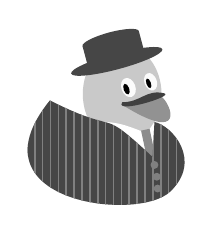
\begin{tikzpicture}[xscale=-1]
	\selectcolormodel{gray}
	\duck[tshirt=white,jacket=brown!50!black,buttons=gray,hat=brown!50!black,tie=brown,stripes={
     \stripes[rotate=0,width=0.02,color=gray,distance=0.1]}]
     \begin{scope}[xshift=62,yshift=1,xscale=-1]
\fill[gray!50!black] (1.8158,1.4731) .. controls (1.5890,1.5312) and (1.5142,1.3598) .. (1.2808,1.3608) .. controls (1.1720,1.2048) and (1.9376,1.4368) .. (1.8158,1.4731) -- cycle;
\end{scope}
\end{tikzpicture}	
	
	
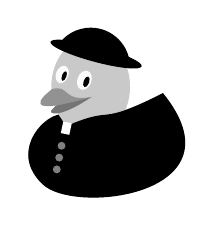
\begin{tikzpicture}
	\selectcolormodel{gray}
	\duck[tshirt=black,buttons=gray,laughing]
 \fill[black, start angle=0, end angle=150, radius=0.5] (1.4,1.75) arc;
   \fill[black,rotate=-15] (0.44,2.1) ellipse (0.6 and 0.1);
	\fill[white,rotate=-12] (0.32,1.) rectangle (0.43,1.15);
\end{tikzpicture}	

	
\end{document}